\chapter{SYSTEM IMPLEMENTATION}
With all the system design and system analysis completed in the previous semester, we now embark on the implementation phase of our project. This chapter details the process of bringing our design to life, outlining the key features of our system and the methodologies employed to implement them. Through careful planning and execution, we aim to translate our theoretical framework into a functional and efficient system. Below are some of the critical features of our system and the approaches we used to implement them.

\section{General Principals and Setups}
\subsection{Frontend}

\subsubsection*{NextJs and App Router}
We created a new Next.js app using the create-next-app command. This command sets up the entire project structure, including necessary configurations and dependencies, making it easier to get started with development.


\subsubsection*{Folder Structure}
\begin{figure}[H]
    \centering
    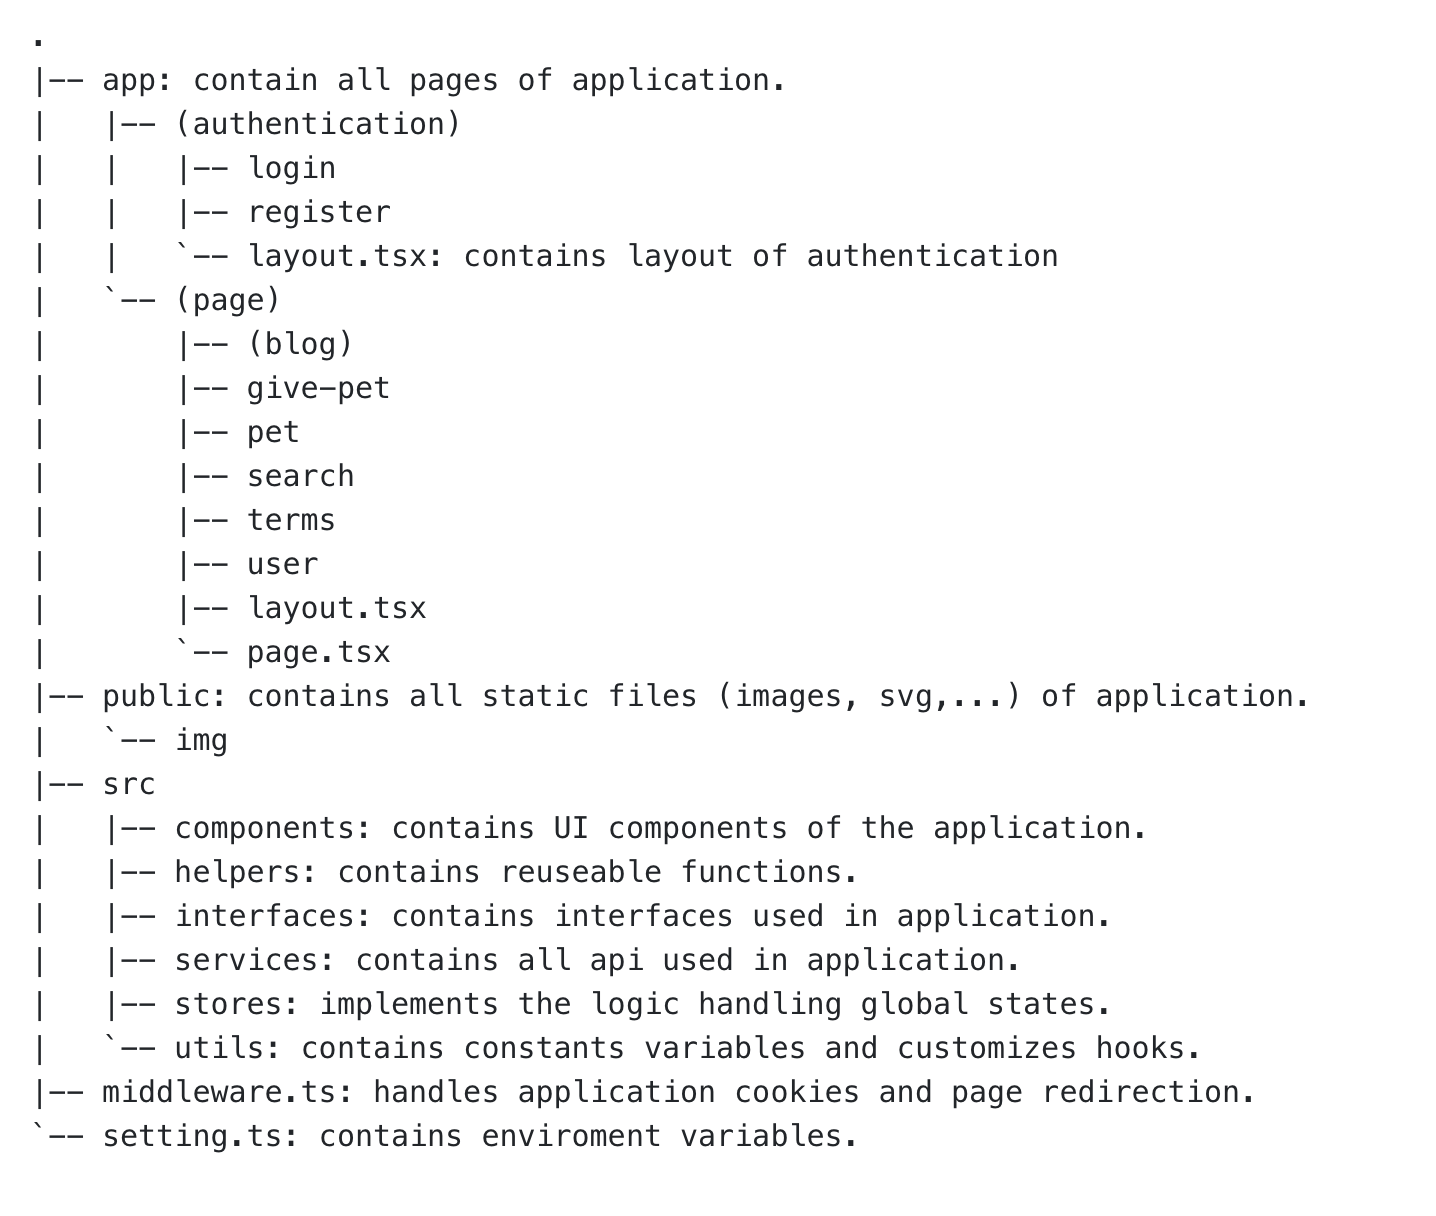
\includegraphics[width=0.8\textwidth]{Figures/Implementation/folder_fe.png}
    \caption{Frontend Folder Structure}
    \label{fig:folder-structure-fe}
\end{figure}

\subsubsection*{Handling Fetching API}

To manage communication with the backend, we developed custom React hooks to handle API requests. These hooks streamline data fetching and modification processes, ensuring efficient and error-free interactions with the backend.

- \textit{useQuery}:

\begin{itemize}
    \item \textbf{Purpose}: To fetch data from the backend.
    \item \textbf{Functionality}: This hook sends a GET request to the API, retrieves data from the database, and handles the loading state and any errors that may occur during the fetch process.
    \item \textbf{Usage Example}:
          \begin{lstlisting}
    const getBlogQuery = useQuery<IApiResponse<IBlogResponse>>(
        [QUERY_KEYS.GET_BLOG_DETAIL, { id: params.id }],
        () => getBlogDetail(params.id),
        {
            onSuccess: (res) => {
            setBlogContent(res.data.data);
            },
            onError: () => {
            // Handle error
            setError(true);
            },
            refetchOnWindowFocus: false,
        }
    );
            \end{lstlisting}
\end{itemize}

- \textit{useMutation}:

\begin{itemize}
    \item \textbf{Purpose}: Modify data, including PUT, POST, and DELETE actions.
    \item \textbf{Functionality}: This hook handles data mutations by sending the appropriate requests to the backend. It manages the state during the request, providing feedback on success or failure, and includes custom error handling.
    \item \textbf{Usage Example}:
          \begin{lstlisting}
    const sendAdoptRequestMutation = useMutation<
        IApiResponse<IUserInfoReponse>,
        IAdoptPetRequest
        >(sendAdoptRequest, {
        onError: () => {
            setAlertMessage('Error sending adoption request');
            setAlertFail(true);
            setAlertShow(true);
        },
        onSuccess: () => {
            setAlertMessage('Adoption request sent successfully');
            setAlertFail(false);
            setAlertShow(true);
        },
        });
            \end{lstlisting}
\end{itemize}

Benefits of using \textit{useQuery} and \textit{useMutation} for API requests:

\begin{itemize}
    \item \textbf{Asynchronous Handling}: Our hooks handle asynchronous operations seamlessly, allowing the frontend to know when data fetching is complete and to take appropriate actions.
    \item \textbf{Error Handling}: Built-in custom error feedback helps identify and address errors effectively.
    \item \textbf{Performance Improvement}: By adding state management during the fetch process, we avoid unnecessary reloads when fetching the same data multiple times.
    \item \textbf{Code Cleanliness}: Using these hooks simplifies the codebase by eliminating repetitive fetch actions, resulting in cleaner and more maintainable code.
\end{itemize}

\subsection{Backend}


\textbf{Folder Structure}

\textbf{Setup Development Environment with Docker}

To start developing the backend, we need to setup the development environment with
all the required components as mentioned in the system architecture, which includes a SQL database, a Redis cache and an Elastic-search database.
\textit{List \ref{lst:docker-code}} show how we install and build all the necessary Docker images to containers.

\begin{lstlisting}[caption=Setup Development Environment with Docker, label={lst:docker-code}]
services:
  database:
    image: mcr.microsoft.com/azure-sql-edge
    container_name: PetopiaDatabase
    ports:
      - "1433:1433"
    env_file:
      - ".env"
    environment:
      ACCEPT_EULA: ${MSSQL_ACCEPT_EULA}
      MSSQL_SA_PASSWORD: ${MSSQL_PASSWORD}
  cache:
    image: redis
    container_name: PetopiaCache
    ports:
      - "6379:6379"
    env_file:
      - ".env"
    command: --requirepass "${REDIS_PASSWORD}"
  searchEngine:
    image: elasticsearch:8.8.1
    container_name: PetopiaSearchEngine
    ports:
      - "9200:9200"
    env_file:
      - ".env"
    environment:
      xpack.security.enabled: ${ELASTIC_SECURITY_ENABLED}
      discovery.type: ${ELASTIC_DISCOVERY_TYPE}
      ELASTIC_PASSWORD: ${ELASTIC_PASSWORD}
\end{lstlisting}

\textbf{Database Implementation with EF Core}

Regarding to implementing the SQL database, we apply the \textit{Code-First} approach following these steps:
\begin{itemize}
    \item Define Domain Entity Classes:
          Start by creating entity classes. These classes represent the tables in the database.

    \item Create a DbContext Class:
          Create a class that extends class DbContext of EF Core. This class represents the database context and provides access to entity classes.

    \item Configure the DbContext:
          Use Fluent API package to configure relationships, keys, and other database-specific settings.

    \item Enable and apply migrations file to create or update the database with the following Linux script:
          \begin{lstlisting}
    dotnet ef migrations add InitialCreate
    dotnet ef database update
  \end{lstlisting}
\end{itemize}

\newpage
\section{Key Feature Implementation}

\subsection{Caching Mechanism}

To reduce the amount of time it takes to access frequently accessed data
and increase the general system performance, we will apply caching data
in our system. The applied caching strategy is called \emph{aside
    caching} \emph{(Figure \ref{fig:caching}).} The detailed caching process is as follows:

- Step 1: The application will check whether the cache has the data it
needs or not.

- Step 2: If the cache has the data the application needs, the process
will end. If the cache has no data, we will go to the next step.

- Step 3: When the cache does not contain the data that the application
needs, the application will go to the database to get the data

- Step 4: The application will save the data retrieved from the database
to the cache, then it will continue its work.

\begin{figure}[H]
    \centering
    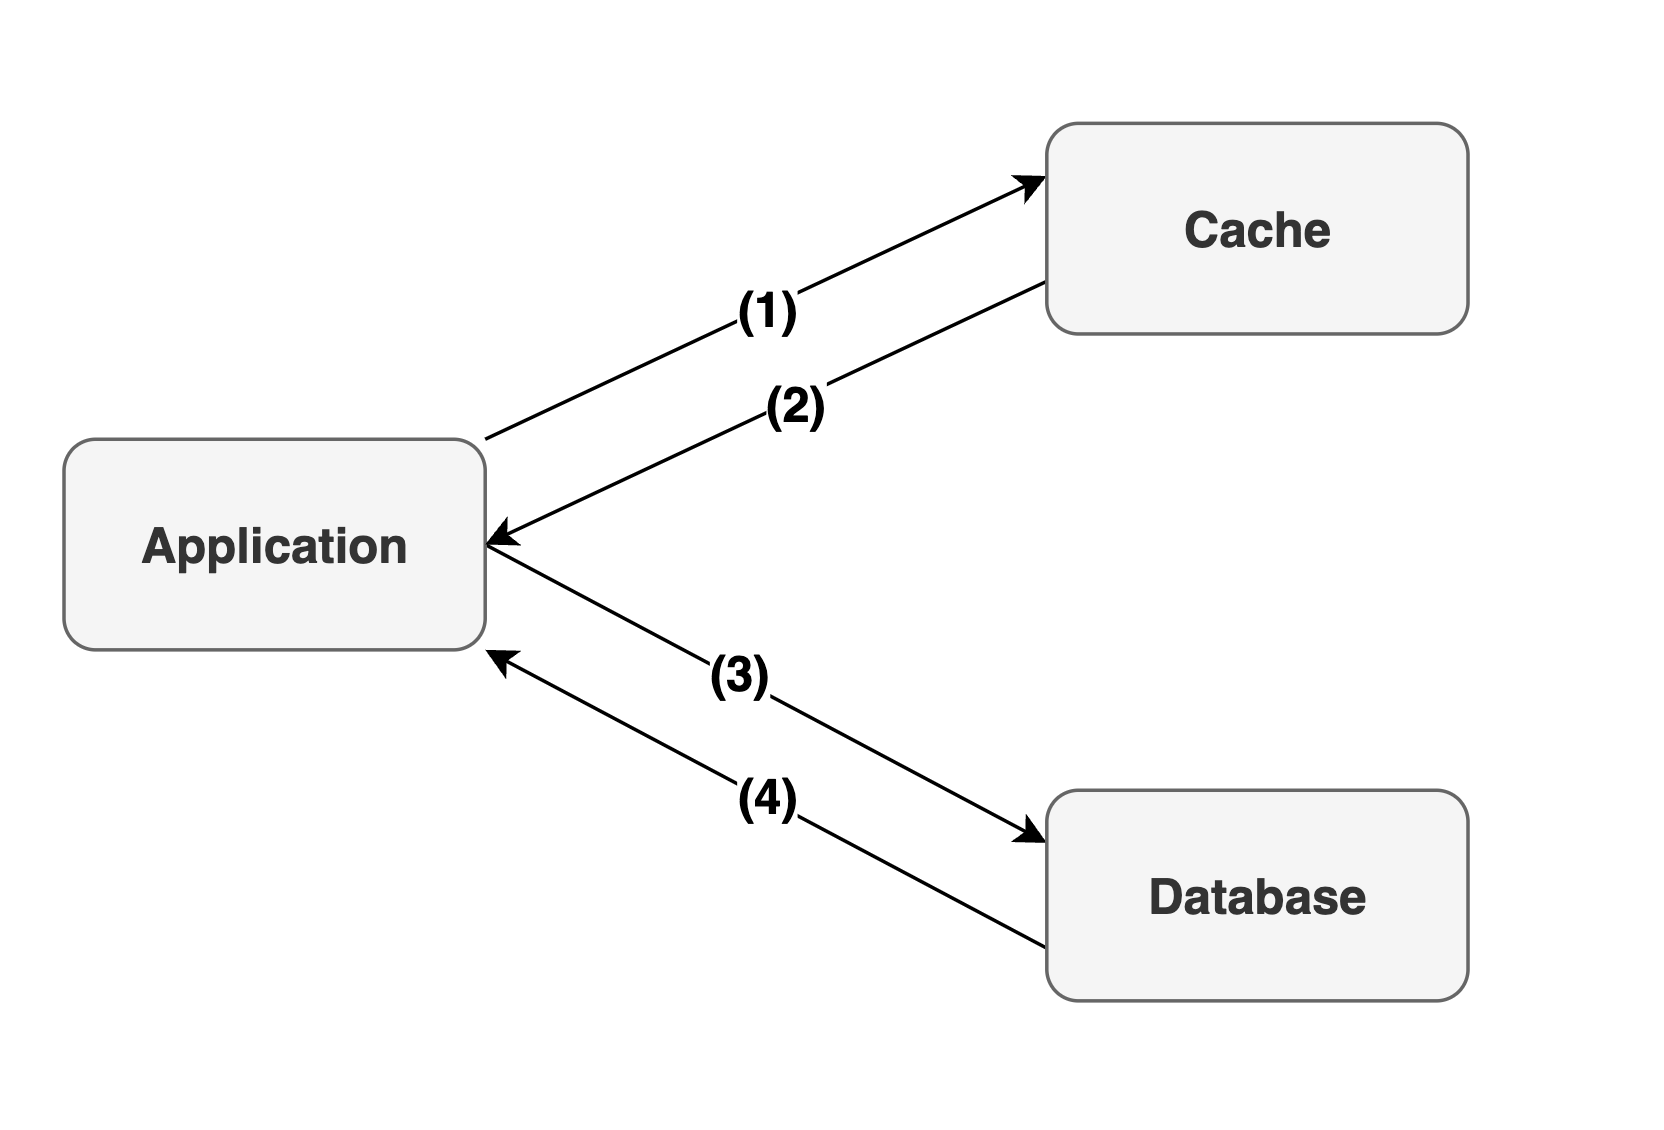
\includegraphics[width=0.8\textwidth]{Figures/caching_strat.png}
    \caption{Caching Mechanism}
    \label{fig:caching}
\end{figure}

\subsection{Advanced search strategy}

Querying data that requires applying many filters (pet profiles, etc)
from the SQL database is extremely time-consuming. Note that only data
that is used repeatedly and is not too large in size can be stored
temporarily in the cache server. Therefore, applying a search strategy
to optimize querying the above type of data is necessary.

\emph{Figure \ref{fig:search-strategy}} shows the steps of syncing data from the SQL database
to the Elastic-search database.

\begin{itemize}
    \item
          Whenever the application does an action on a record of the SQL
          database (create, update, delete), a new record (which includes the ID
          of the record taken the action, and the action), from now we call the
          async record, is created.
    \item
          At the end of the application process, a background job is triggered
          to query all the async records and send all the records that they
          point to onto the Elastic-search database. Therefore the data of the
          Elastic-search database is always synchronized with the SQL database.
    \item
          Note that the application only queries data from the Elastic-search
          database for tables that were defined before.
\end{itemize}

\begin{figure}[H]
    \centering
    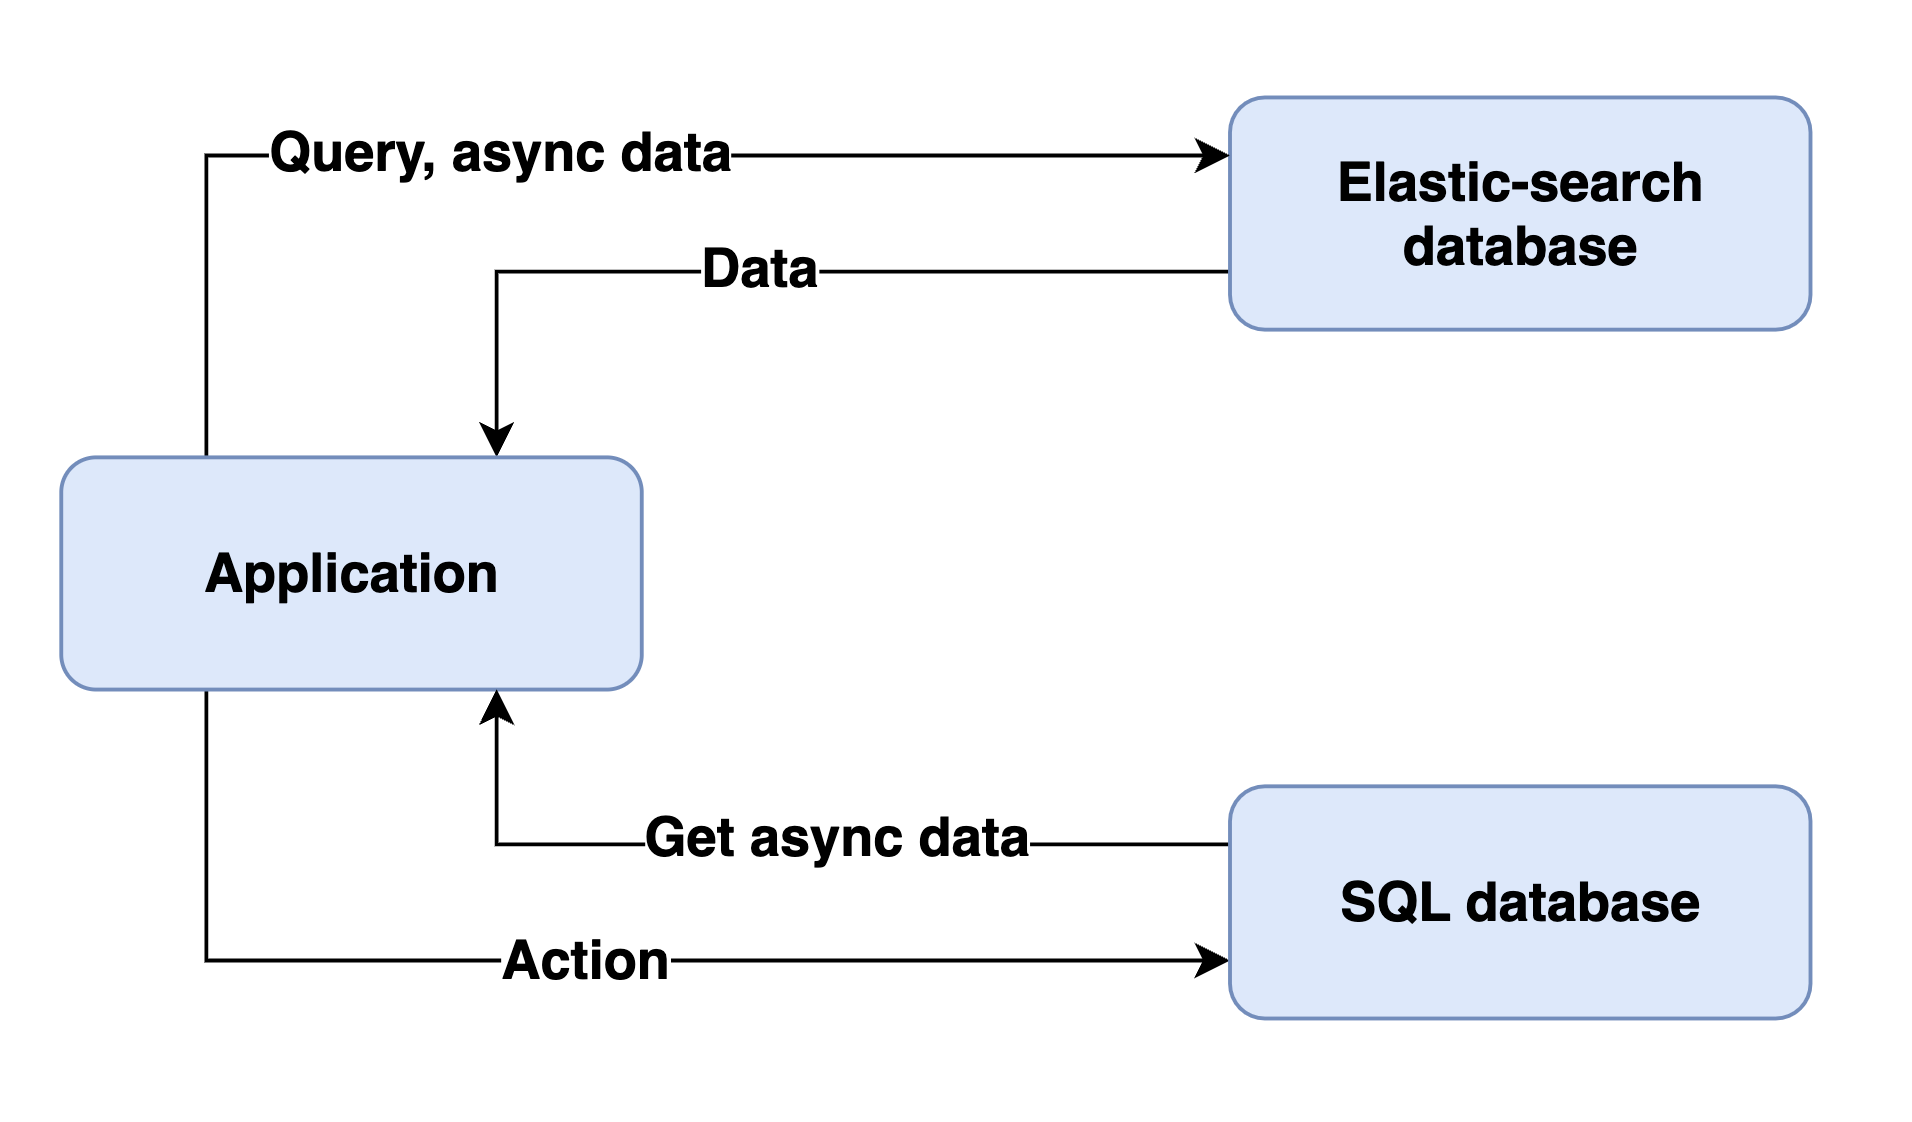
\includegraphics[width=0.8\textwidth]{Figures/search_strat.png}
    \caption{Search strategy}
    \label{fig:search-strategy}
\end{figure}

\subsection{Online payment}

In our system, we have integrated the PayPal Braintree Gateway to handle online payments securely and efficiently. Braintree is a full-stack payment platform that offers a seamless payment experience, supporting various payment methods, including credit cards, PayPal, and other digital wallets. Its robust infrastructure and comprehensive SDKs for both client and server sides make it an ideal choice for our system's payment processing needs.

\begin{figure}[H]
    \centering
    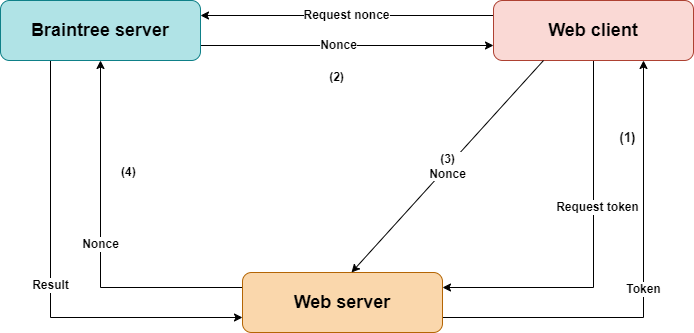
\includegraphics[width=0.7\textwidth]{Figures/payment-strat.png}
    \caption{Payment process}
    \label{fig:payment-flow}
\end{figure}

\emph{Figure \ref{fig:payment-flow}} breaks down how the payment process is implemented:

- Step 1:
The front-end requests a client token from our server and initializes the Braintree client. This token is essential for securely communicating between the client and the Braintree server.\\
Our server generates a client token using Braintree's tools and sends it back to the client. This token allows the front-end to securely handle customer payment information.

- Step 2:
The customer enters their payment information on the front-end. The Braintree client communicates this information to Braintree and returns a payment method nonce, a secure reference representing the payment details.

- Step 3:
The front-end sends the payment method nonce to our server. This nonce is a secure way to pass payment information without exposing sensitive data.

- Step 4:
The server receives the payment method nonce and uses Braintree's tools to process the payment. The server then communicates with Braintree to complete the transaction securely.

By utilizing PayPal Braintree Gateway, we ensure a secure and streamlined payment process, enhancing the user experience and maintaining high security standards in handling sensitive payment information.

\subsection{Google Login}
Our website provides users with the option to log in using their Google account,
offering a convenient and secure authentication method. By integrating Google Sign-In,
we simplify the login process for users and enhance the overall user experience.

The Google Login process is illustrated in \emph{Figure \ref{fig:gglogin-flow}}:
\begin{figure}[H]
    \centering
    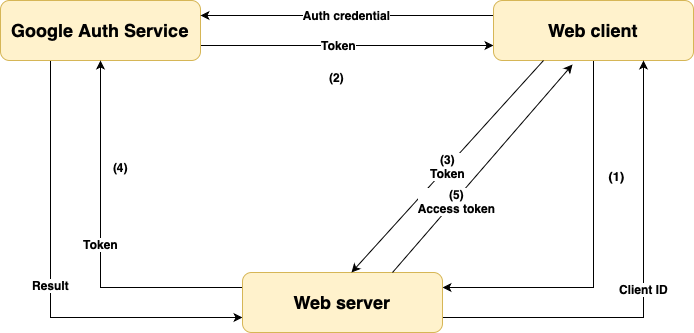
\includegraphics[width=0.7\textwidth]{Figures/Implementation/GoogleLogin.png}
    \caption{Google Login Process}
    \label{fig:gglogin-flow}
\end{figure}

The implementation steps are as follows:
\begin{itemize}
    \item Step 1: The web client obtains the client ID from the web server.
    \item Step 2: When the user clicks the Google login button, the web client displays the Google Login form. The user logs in using their Google account, and Google generates a token, which is sent back to the web client.
    \item Step 3: The web client sends the token to the web server.
    \item Step 4: The web server verifies the token with Google. If the token is valid, Google confirms this to the web server.
    \item Step 5: The web server creates an access token and sends it back to the web client. The user can now access the website using this access token.
\end{itemize}

\subsection{Breeds Recognition}
Breed recognition is a valuable feature for our users, who often don't know their pet's breed. To address this, we utilized ML.NET
to train an image classification model. This advanced technology enables our platform to accurately identify a pet's breed from a photo,
simplifying the process for users and enhancing their experience.

The first step is preparing the dataset. We have chosen the Stanford Dogs dataset\footnote{Stanford Dogs dataset: \url{https://www.kaggle.com/datasets/jessicali9530/stanford-dogs-dataset}}, which contains images of 120 dog breeds from around
the world. This dataset, built using images and annotations from ImageNet, is ideal for the task of fine-grained image categorization.
The challenging nature of this problem stems from the fact that certain dog breeds have nearly identical features or differ only in color and age.

For cat breed classification, we use the Cat Breeds Dataset (Cleared)\footnote{Cat Breeds Dataset (Cleared): \url{https://www.kaggle.com/datasets/denispotapov/cat-breeds-dataset-cleared}}, which contains images of 67 different cat breeds, labeled by advertisers for
adoption. This dataset is a refined version of the original Cat Breeds Dataset from Kaggle \footnote{Stanford Dogs dataset: \url{https://www.kaggle.com/ma7555/cat-breeds-dataset}}.
The cleared version has been meticulously cleaned to remove non-cat images, indistinguishable cat photos, duplicates, and very small images
(height or width less than 150 pixels). This ensures that the dataset is of high quality, facilitating accurate training and performance of our
machine learning model.

The images in the dataset are organized into separate folders for each dog breed, simplifying the model training process. This organization
makes it more convenient to manage and feed the data into our machine learning model. Using this well-structured dataset, we can effectively
train our image classification model with ML.NET to recognize and categorize various dog breeds accurately.

The next step involves using ML.NET Model Builder to transform our image set into an image classification model. Here's how we proceed:
\begin{enumerate}
    \item Load the Data: Import the cleaned datasets for dog and cat breeds into the ML.NET Model Builder. These datasets include images
          categorized into folders based on their respective breeds.
    \item Set Up the Environment: Configure the Model Builder environment on our local machine, ensuring that all necessary tools and dependencies are installed.
    \item Select the Scenario: Choose the 'Image Classification' scenario in ML.NET Model Builder, which is specifically designed for tasks like breed recognition.
    \item Train the Model:
          \begin{itemize}
              \item Data Preprocessing: The Model Builder automatically preprocesses the images, resizing and normalizing them as required.
              \item Model Selection and Training: The tool selects a suitable pre-trained model and fine-tunes it using our dataset. This involves
                    splitting the data into training and validation sets to ensure the model learns effectively and generalizes well.
              \item Local Training: The model is trained on our local machine, leveraging available computational resources to iterate through
                    the dataset and optimize the classification accuracy.
          \end{itemize}
    \item Evaluate the Model: Once training is complete, the Model Builder evaluates the model's performance,
          providing metrics such as accuracy, precision, recall, and F1 score. This helps in understanding how well
          the model distinguishes between different breeds.

          After training the model for dog breed recognition, we evaluated its performance using various algorithms.
          The micro-accuracy algorithm identified the best model, achieving a micro-accuracy score of 0.8345. This
          high accuracy indicates that the model can reliably recognize and classify different dog breeds, providing
          users with accurate breed identification based on their pet's images.

          \begin{figure}[H]
              \centering
              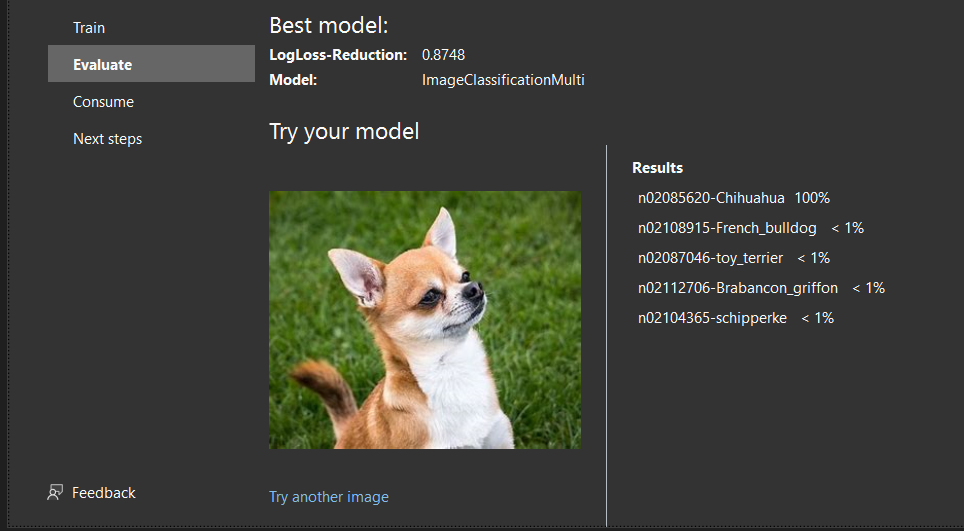
\includegraphics[width=0.7\textwidth]{Figures/AI/ai_result.png}
              \caption{Results of Dog Breed Recognition}
          \end{figure}

          For cat breed recognition, we followed a similar process, training the model on the Cat Breeds Dataset (Cleared)
          and evaluating its performance. The micro-accuracy algorithm identified the best model, achieving a micro-accuracy
          score of 0.4321. This indicates that the dataset is more challenging for cat breed recognition, as the model's accuracy
          is lower compared to dog breed recognition. Despite this, the model can still classify cat breeds with reasonable accuracy,
          providing users with valuable insights into their pet's breed based on images.

    \item Export the Model: Finally, the trained model is exported for integration into our application.
          The Model Builder generates the necessary code and files, making it straightforward to deploy the model.
          In our case, we export the model as an API, allowing seamless integration with our platform for real-time breed recognition.
\end{enumerate}

\subsection{Protect System APIs with Access/Refresh Tokens}
To authenticate users and authorize requests without keeping session data on the server, we use \textit{tokens}, which are data confirming a user’s identity and are analogous to digital signatures.

A careful balance between security and user experience is essential for authentication and authorization. A user may become irritated if protocols are overly strict. On the other hand, a security breach is imminent if permission systems are too loose. Access and refresh tokens provide a solution that meets both requirements.

\textbf{An access token} allows temporary access to restricted resources such as APIs or websites. The chance of the access token being compromised or stolen increases the longer it’s valid. Therefore, access tokens are valid for only \textit{a few minutes or hours}.

\textbf{A refresh token} allow developers to manage users’ sessions across the application. Additionally, they allow users to log in and stay connected without providing their passwords for long periods. Therefore, refresh tokens can last \textit{from a few days to a few months}.

Let’s now discuss how to set up the tokens in \textit{Figure \ref{fig:tokens-flow}}.

Let’s say a client requests an access token by authenticating with the authorization server and delivering a credential that proves the resource owner is authorized to use the resource.

The API server verifies the authorization and confirms the identity of the authorized client. An access token and a refresh token are issued if it’s legitimate. The client must securely store this refresh token.

The client can now request the API server for secured resource access, and the resource server validates the access token. If it’s valid, it returns the desired resource.

\begin{figure}[H]
    \centering
    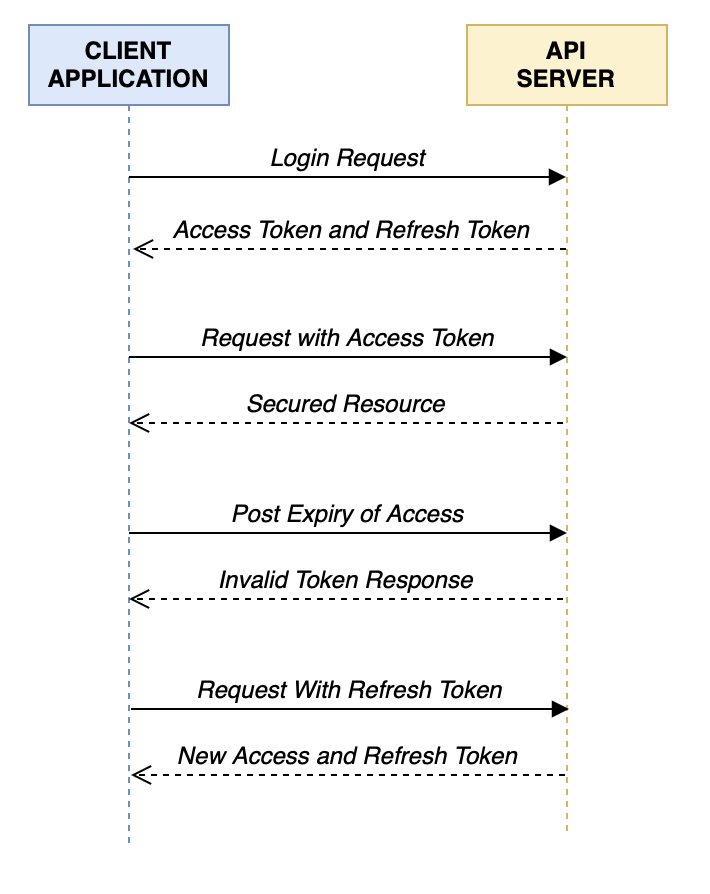
\includegraphics[width=0.6\textwidth]{Figures/Implementation/Tokens.png}
    \caption{Set up the tokens.}
    \label{fig:tokens-flow}
\end{figure}

\subsection{Back Office Implementation with Retool}
To build the back office web-based application for administration functionality, we use Retool and follow these steps:
\begin{itemize}
    \item Connect Data Sources: Start by creating a resource in Retool, we connect our MSSQL Database Server to Retool.
          This step ensures that our dashboard can pull in data from the database.
    \item Design Dashboard: Retool provides a drag-and-drop interface for building custom admin dashboards.
          We can find components like tables, buttons, text inputs, and dropdowns.
          These components are essential for displaying data, triggering actions, and interacting with users.
    \item Customize Styles and Triggers: We customize the appearance of dashboard components by adjusting styles.
          Additionally, we set up triggers to respond to user interactions, such as button clicks or form submissions.
    \item Test and Iterate: We assemble our dashboard, test it thoroughly, and iterate based on testing feedback.
\end{itemize}

Retool enables rapid development process, letting us move quickly from requirements to implementation. Also, Retool provides us a free hosting cloud, eliminating the need for complex infrastructure
management. Nevertheless, because of modifying directly the database instead of utilizing the API Server, the system cannot
catch those database changes normally and process further actions after those database changes. Therefore, it is a need for handling this disavantages.
A proposed solution will be discussed in the next section.

\subsection{Background Task Processing}
As for features require tasks with huge processing time or(and) running many times on the specified CRON (Linux command-line utility for scheduling tasks) schedule,
we should perform them separately from the main process of the application or the process of each API request.

In ASP.NET, for handling this problem, we use \textit{Hangfire}, an open-source framework, to create process and manage our background jobs.

\textbf{Sending Emails and Synchronizing Elastic-search Records}

The \textit{Fire-and-forget} technique is applied to sending emails and synchronizing Elastic-search records.
In this technique, we create a background job, let it run only once and imediately after the creation.
Hangfire framework helps us to check if the job is successfully terminated. In the case of failure, automatically, Hangfire will re-create and
run a new background job. Thus, we can reduce the response time of requests from web clients, prevent bottleneck and ensure the correct operation of the system.

\textbf{Scheduly Handling Update Account Requests}

Hangfire framework supports us \textit{Recurring Jobs} to handle scheduling tasks.
As mentioned before, in our system, when admins confirm a user to be upgraded to an organization or create a new admin,
the back office will directly modify tables in the MSSQL Database Server.
Therefore, recurring jobs are helpful to the API Server for catching those modifications in the database server
(by checking the database scheduly) and processing any further actions such as sending notication emails to
users.